%%%%%%%%%%%%%%%%%%%%%%%%
%
% $Autor: Hemanth Jadiswami Prabhakaran $
% $Datum: 2025-06-30 11:19:39Z $
% $Pfad: GitHub/BA25-01-Time-Series/Manual/Chapters/en/08Troubleshooting.tex $
% $Version: 1 $
%
% $Project: BA25-Time-Series $
%
%%%%%%%%%%%%%%%%%%%%%%%%



\chapter{Troubleshooting}

\section{Troubleshooting Framework}

This chapter provides comprehensive problem resolution procedures for the Walmart Sales Forecasting System. It covers common issues, diagnostic procedures, and systematic approaches to resolving problems in both local and cloud deployments.



\section{Installation and Setup Issues}

\subsection{Python Version Problems}

\subsubsection{Wrong Python Version}

\textbf{Problem}: System reports Python version other than 3.12.x

\textbf{Symptoms}:
\begin{itemize}
	\item Package installation failures
	\item Import errors when running applications
	\item Virtual environment creation errors
	\item Dependency conflict messages
\end{itemize}

\textbf{Diagnostic Steps}:
\begin{lstlisting}[language=bash,basicstyle=\color{blue}]
	# Check current Python version
	python --version
	python3 --version
	
	# Check which Python executable is being used
	which python
	which python3
	
	# List all available Python versions
	ls /usr/bin/python*  # Linux/macOS
\end{lstlisting}

\textbf{Solution}:
\begin{enumerate}
	\item Download Python 3.12.x from \url{https://www.python.org/downloads/}
	\item Install the correct version
	\item Use explicit version commands:
	\begin{lstlisting}[language=bash]
		# Use specific Python version
		python3.12 -m venv walmart_forecast_env
		python3.12 -m pip install -r requirements.txt
	\end{lstlisting}
	\item Update system PATH if necessary
\end{enumerate}


\subsubsection{Multiple Python Installations}

\textbf{Problem}: Conflicts between different Python installations

\textbf{Symptoms}:
\begin{itemize}
	\item Inconsistent behavior between terminals
	\item Package installed but not found
	\item Virtual environment using wrong Python version
\end{itemize}

\textbf{Solution}:
\begin{lstlisting}[language=bash,basicstyle=\color{blue}]
	# Explicitly specify Python executable
	/usr/bin/python3.12 -m venv walmart_forecast_env
	
	# Or use pyenv for version management (recommended)
	pyenv install 3.12.0
	pyenv local 3.12.0
	python -m venv walmart_forecast_env
\end{lstlisting}

\subsection{Virtual Environment Issues}

\subsubsection{Environment Activation Failures}

\textbf{Problem}: Virtual environment won't activate

\textbf{Symptoms}:
\begin{itemize}
	\item "No such file or directory" errors
	\item Activation script not found
	\item Permission denied errors
\end{itemize}

\textbf{Diagnostic Steps}:
\begin{lstlisting}[language=bash,basicstyle=\color{blue}]
	# Check if virtual environment directory exists
	ls -la walmart_forecast_env/
	
	# Check activation script
	ls -la walmart_forecast_env/bin/activate  # Linux/macOS
	ls -la walmart_forecast_env\Scripts\activate.bat  # Windows
	
	# Check permissions
	ls -la walmart_forecast_env/bin/
\end{lstlisting}

\textbf{Solution}:
\begin{lstlisting}[language=bash,basicstyle=\color{blue}]
	# Recreate virtual environment
	rm -rf walmart_forecast_env
	python3.12 -m venv walmart_forecast_env
	
	# Fix permissions if needed (Linux/macOS)
	chmod +x walmart_forecast_env/bin/activate
	
	# Use alternative activation method
	source walmart_forecast_env/bin/activate
	# or
	. walmart_forecast_env/bin/activate
\end{lstlisting}

\subsection{Dependency Installation Problems}

\subsubsection{Package Installation Failures}

\textbf{Problem}: pip install fails for required packages

\textbf{Symptoms}:
\begin{itemize}
	\item Build errors during installation
	\item "No module named" errors after installation
	\item Version conflict messages
	\item SSL certificate errors
\end{itemize}

\textbf{Diagnostic Steps}:
\begin{lstlisting}[language=bash,basicstyle=\color{blue}]
	# Check pip version
	pip --version
	
	# Verify virtual environment is active
	which pip
	which python
	
	# Check for conflicting packages
	pip check
	
	# Try manual installation of problematic package
	pip install -v package_name
\end{lstlisting}

\textbf{Solution}:
\begin{lstlisting}[language=bash,basicstyle=\color{blue}]
	# Upgrade pip first
	pip install --upgrade pip
	
	# Clear pip cache
	pip cache purge
	
	# Install with specific options
	pip install --no-cache-dir -r requirements.txt
	
	# For SSL issues
	pip install --trusted-host pypi.org --trusted-host pypi.python.org -r requirements.txt
	
	# Install packages one by one to identify problem
	pip install streamlit==1.32.0
	pip install pandas==2.2.2
	# ... continue with each package
\end{lstlisting}


\section{Application Launch Issues}

\subsection{Streamlit Startup Problems}

\subsubsection{Port Already in Use}

\textbf{Problem}: "Address already in use" error when launching

\textbf{Symptoms}:
\begin{itemize}
	\item Error: "OSError: [Errno 48] Address already in use"
	\item Application won't start
	\item Previous sessions still running
\end{itemize}

\textbf{Diagnostic Steps}:
\begin{lstlisting}[language=bash,basicstyle=\color{blue}]
	# Check what's using the port
	lsof -i :8501  # Linux/macOS
	netstat -ano | findstr :8501  # Windows
	
	# List all Streamlit processes
	ps aux | grep streamlit  # Linux/macOS
	tasklist | findstr streamlit  # Windows
\end{lstlisting}

\textbf{Solution}:
\begin{lstlisting}[language=bash,basicstyle=\color{blue}]
	# Kill existing Streamlit processes
	pkill -f streamlit  # Linux/macOS
	taskkill /F /IM python.exe  # Windows (be careful!)
	
	# Or use different port
	streamlit run walmartSalesTrainingApp.py --server.port=8503
	streamlit run walmartSalesPredictionApp.py --server.port=8504
	
	# Or specify port in command
	streamlit run app.py --server.port=8502
\end{lstlisting}

\subsubsection{Import Errors on Startup}

\textbf{Problem}: Module import errors when launching applications

\textbf{Symptoms}:
\begin{itemize}
	\item "ModuleNotFoundError" messages
	\item "ImportError" for specific packages
	\item Application crashes immediately
\end{itemize}

\textbf{Diagnostic Steps}:
\begin{lstlisting}[language=bash,basicstyle=\color{blue}]
	# Test imports manually
	python -c "import streamlit; print('Streamlit OK')"
	python -c "import pandas; print('Pandas OK')"
	python -c "import plotly; print('Plotly OK')"
	
	# Check installed packages
	pip list | grep streamlit
	pip show streamlit
\end{lstlisting}

\textbf{Solution}:
\begin{lstlisting}[language=bash,basicstyle=\color{blue}]
	# Reinstall problematic packages
	pip uninstall streamlit
	pip install streamlit==1.32.0
	
	# Verify virtual environment is active
	echo $VIRTUAL_ENV
	
	# Reinstall all dependencies
	pip install --force-reinstall -r requirements.txt
\end{lstlisting}

\section{Cloud Application Issues}

\subsection{Cloud Access Problems}

\subsubsection{Application Won't Load}

\textbf{Problem}: Cloud application shows loading screen indefinitely

\textbf{Symptoms}:
\begin{itemize}
	\item Endless "Please wait..." message
	\item White screen after initial load
	\item Browser shows "Connection timed out"
\end{itemize}

\textbf{Diagnostic Steps}:
\begin{enumerate}
	\item Check internet connection stability
	\item Try different browser (Chrome recommended)
	\item Check browser console for errors (F12)
	\item Test with incognito/private browsing mode
\end{enumerate}

\textbf{Solution}:
\begin{enumerate}
	\item Refresh the page (Ctrl+F5 for hard refresh)
	\item Clear browser cache and cookies
	\item Disable browser extensions temporarily
	\item Try different network connection
	\item Wait 5-10 minutes and retry (server may be busy)
\end{enumerate}



\subsubsection{Session Timeout Issues}

\textbf{Problem}: Application resets unexpectedly

\textbf{Symptoms}:
\begin{itemize}
	\item Loaded models disappear
	\item Interface resets to initial state
	\item "Please rerun" messages appear
\end{itemize}

\textbf{Solution}:
\begin{itemize}
	\item Be aware of 30-minute idle timeout
	\item Save/download results frequently
	\item Keep browser tab active
	\item Refresh page to restart session
	\item Use local installation for long training sessions
\end{itemize}

\subsection{File Upload Problems}

\subsubsection{Upload Failures}

\textbf{Problem}: File uploads fail or hang

\textbf{Symptoms}:
\begin{itemize}
	\item Upload progress bar stuck
	\item "File too large" errors
	\item Upload completes but file not recognized
\end{itemize}

\textbf{Diagnostic Steps}:
\begin{enumerate}
	\item Check file size (must be < 200MB for cloud)
	\item Verify file format (.csv for data, .pkl for models)
	\item Test with smaller sample file
	\item Check network connection stability
\end{enumerate}

\textbf{Solution}:
\begin{enumerate}
	\item Compress large files or reduce dataset size
	\item Ensure files are saved in correct format
	\item Try upload during off-peak hours
	\item Use local installation for large files
	\item Split large datasets into smaller chunks
\end{enumerate}

\section{Data-Related Issues}

\subsection{Data Format Problems}

\subsubsection{CSV Schema Errors}

\textbf{Problem}: Data files don't meet required schema

\textbf{Symptoms}:
\begin{itemize}
	\item "Missing required column" errors
	\item "Data type mismatch" warnings
	\item Processing fails after upload
\end{itemize}

\textbf{Required Schema Validation}:
\begin{lstlisting}[language=python]
vs
\end{lstlisting}

\textbf{Solution}:
\begin{enumerate}
	\item Verify all required columns are present
	\item Check column names for exact spelling and capitalization
	\item Ensure date format is YYYY-MM-DD
	\item Validate numeric columns contain only numbers
	\item Remove any extra columns not required by schema
\end{enumerate}

\begin{figure}[H]
	\centering
	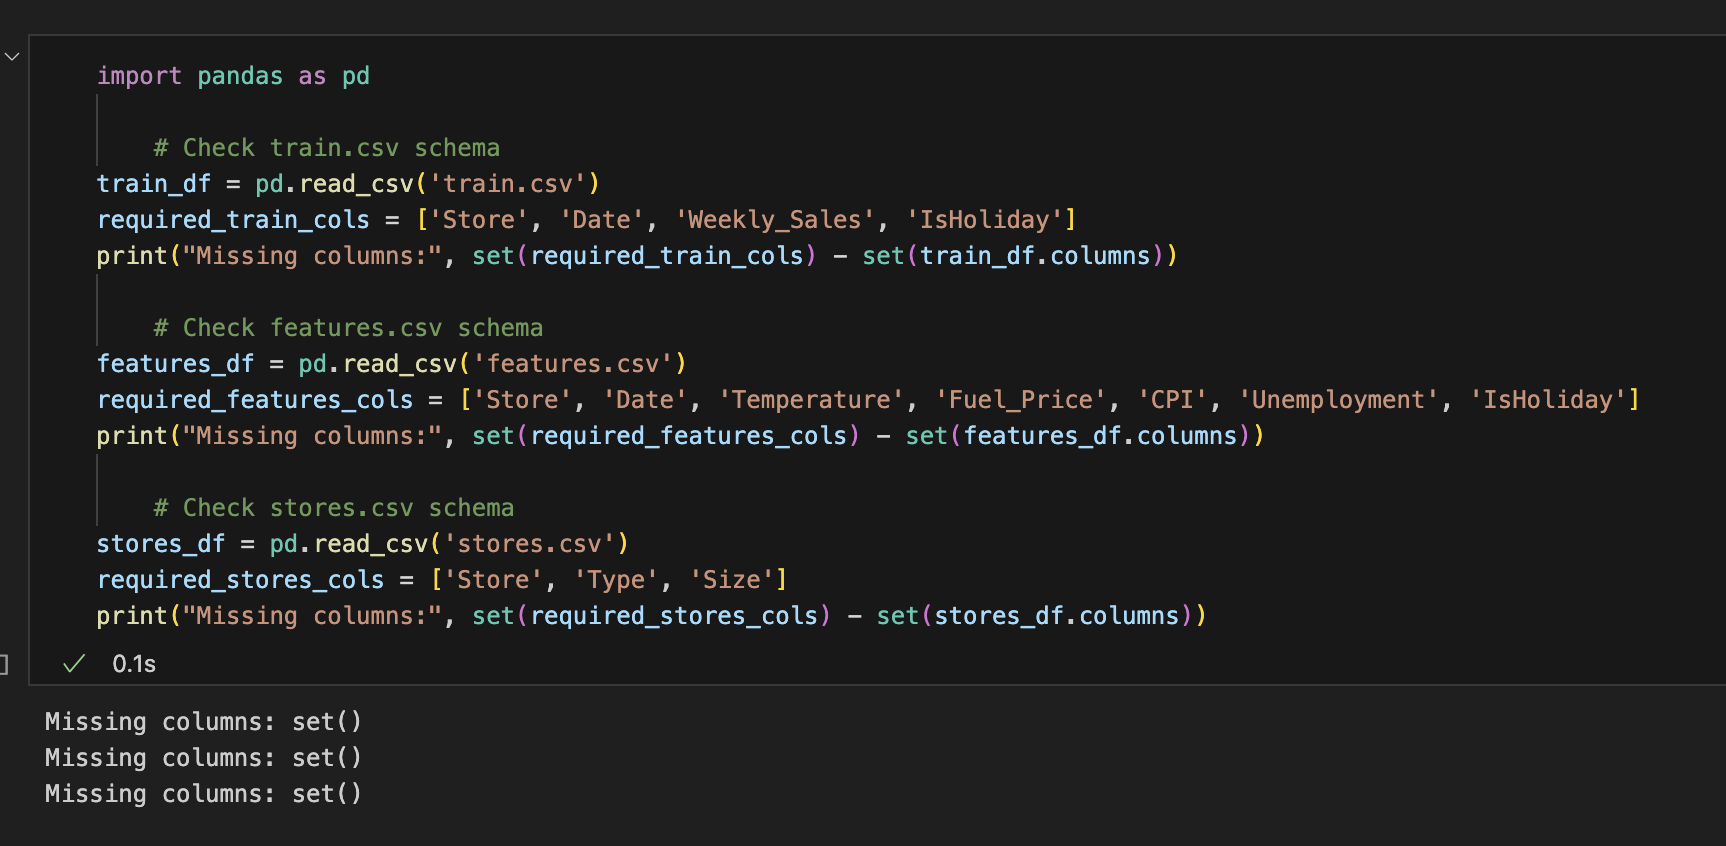
\includegraphics[width=0.9\textwidth]{Images/08Troubleshooting/DataSchemaValidation.png}
	\caption{Data Schema Validation Error Resolution}
	\label{fig:data_schema_validation}
\end{figure}

\subsubsection{Data Quality Issues}

\textbf{Problem}: Data contains invalid or inconsistent values

\textbf{Symptoms}:
\begin{itemize}
	\item Training fails with "Invalid data" errors
	\item Negative sales values causing rejection
	\item Date parsing errors
	\item Store ID mismatches between files
\end{itemize}

\textbf{Data Quality Validation}:
\begin{lstlisting}[language=python,basicstyle=\color{blue}]
	# Check for negative sales
	negative_sales = train_df[train_df['Weekly_Sales'] < 0]
	print(f"Negative sales records: {len(negative_sales)}")
	
	# Check date format consistency
	try:
	pd.to_datetime(train_df['Date'])
	print("Date format OK")
	except:
	print("Date format issues detected")
	
	# Check Store ID consistency
	train_stores = set(train_df['Store'].unique())
	features_stores = set(features_df['Store'].unique())
	stores_stores = set(stores_df['Store'].unique())
	print("Store ID mismatches:", train_stores.symmetric_difference
	(features_stores))
\end{lstlisting}

\begin{figure}[H]
	\centering
	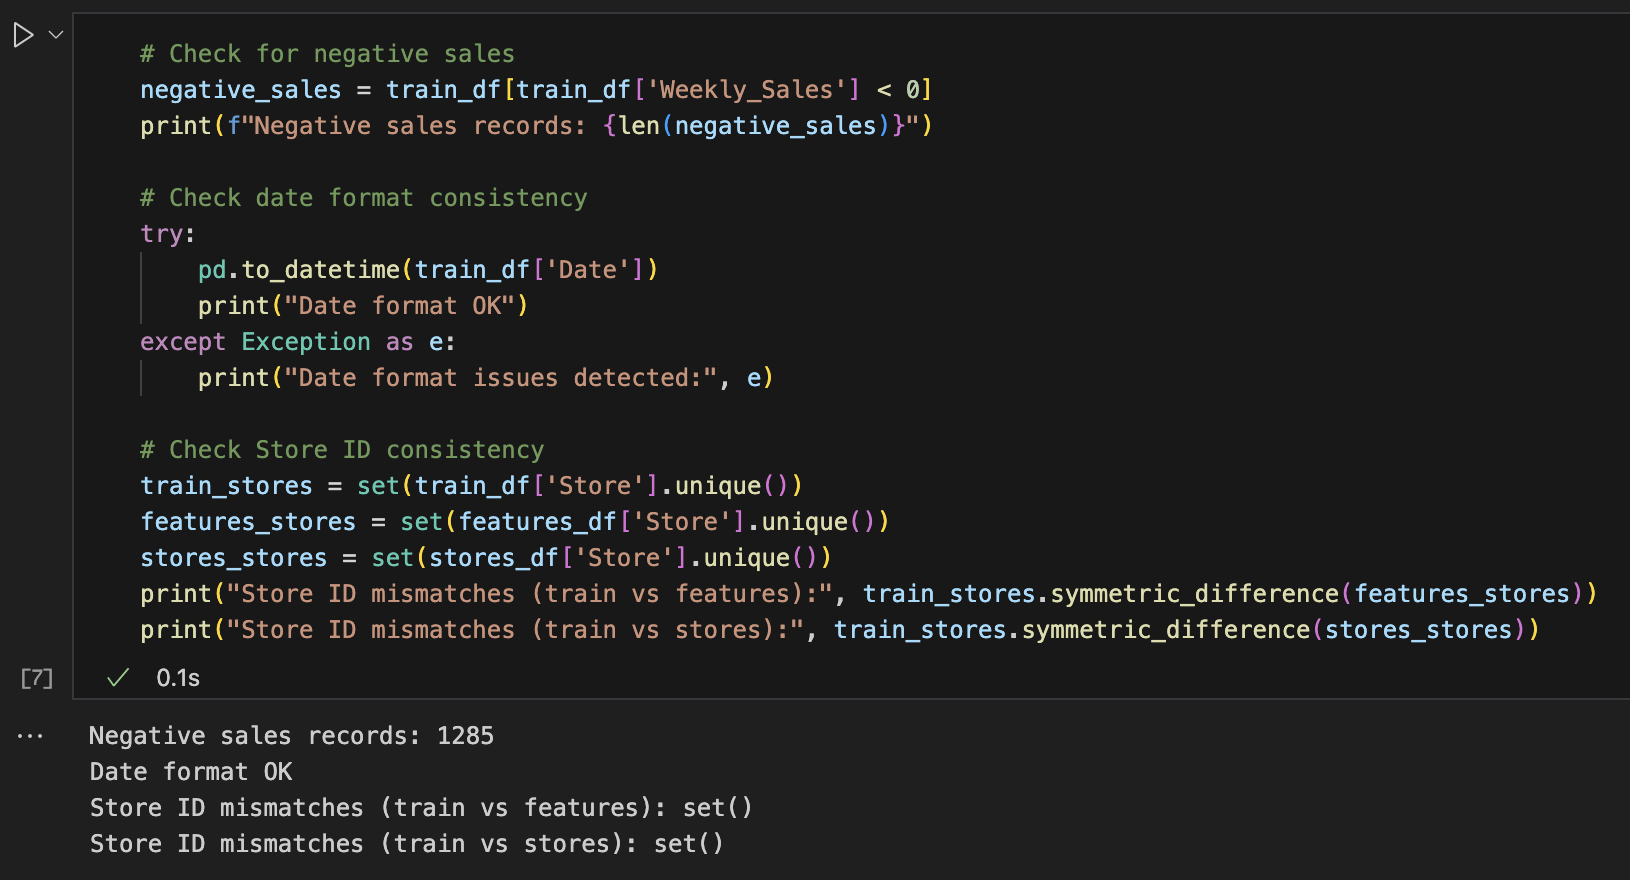
\includegraphics[width=0.9\textwidth]{Images/08Troubleshooting/DataQualityValidation.png}
	\caption{Data Schema Validation Error Resolution}
	\label{fig:data_quality_validation}
\end{figure}

\textbf{Solution}:
\begin{enumerate}
	\item Remove or correct negative sales values
	\item Standardize date formats to YYYY-MM-DD
	\item Ensure Store IDs match across all files
	\item Fill missing values appropriately
	\item Validate data ranges are reasonable
\end{enumerate}

\subsection{Model Compatibility Issues}

\subsubsection{Model Loading Failures}

\textbf{Problem}: Custom models fail to load

\textbf{Symptoms}:
\begin{itemize}
	\item "Invalid model file" errors
	\item "Model format not supported" messages
	\item Application crashes when loading model
\end{itemize}

\textbf{Diagnostic Steps}:
\begin{lstlisting}[language=python,basicstyle=\color{blue}]
	import joblib
	import pickle
	
	# Test model file integrity
	try:
	model = joblib.load('model.pkl')
	print("Joblib loading successful")
	except Exception as e:
	print(f"Joblib error: {e}")
	
	try:
	with open('model.pkl', 'rb') as f:
	model = pickle.load(f)
	print("Pickle loading successful")
	except Exception as e:
	print(f"Pickle error: {e}")
\end{lstlisting}

\textbf{Solution}:
\begin{enumerate}
	\item Ensure model was trained with Python 3.12
	\item Verify model type matches selection (ARIMA vs Exponential Smoothing)
	\item Retrain model if cross-platform compatibility issues
	\item Check file wasn't corrupted during transfer
	\item Use same package versions for training and prediction
\end{enumerate}

\section{Performance Issues}

\subsection{Slow Training Performance}

\subsubsection{Training Takes Too Long}

\textbf{Problem}: Model training exceeds expected time

\textbf{Symptoms}:
\begin{itemize}
	\item Auto ARIMA takes hours instead of minutes
	\item Application becomes unresponsive
	\item Memory usage continuously increases
\end{itemize}

\textbf{Diagnostic Steps}:
\begin{lstlisting}[language=python,basicstyle=\color{blue}]
	import psutil
	import time
	
	# Monitor system resources
	def monitor_resources():
	process = psutil.Process()
	while True:
	cpu_percent = process.cpu_percent()
	memory_mb = process.memory_info().rss / 1024 / 1024
	print(f"CPU: {cpu_percent}%, Memory: {memory_mb:.1f}MB")
	time.sleep(10)
\end{lstlisting}

\textbf{Solution}:
\begin{enumerate}
	\item Reduce hyperparameter search space:
	\begin{lstlisting}[language=python]
		# Use smaller parameter ranges
		max_p = 5  # instead of 20
		max_q = 5  # instead of 20
	\end{lstlisting}
	\item Use smaller dataset for initial testing
	\item Increase system RAM if possible
	\item Use stepwise ARIMA search instead of exhaustive
	\item Consider Exponential Smoothing for faster training
\end{enumerate}

\subsection{Memory Issues}

\subsubsection{Out of Memory Errors}

\textbf{Problem}: Application runs out of memory during training

\textbf{Symptoms}:
\begin{itemize}
	\item "MemoryError" exceptions
	\item System becomes slow and unresponsive
	\item Training process killed by OS
\end{itemize}

\textbf{Solution}:
\begin{lstlisting}[language=python,basicstyle=\color{blue}]
	# Implement data chunking
	def process_in_chunks(data, chunk_size=10000):
	for i in range(0, len(data), chunk_size):
	chunk = data[i:i+chunk_size]
	# Process chunk
	yield chunk
	
	# Force garbage collection
	import gc
	gc.collect()
	
	# Use memory-efficient data types
	df = df.astype({
		'Store': 'int16',
		'Weekly_Sales': 'float32'
	})
\end{lstlisting}

\begin{figure}[H]
	\centering
	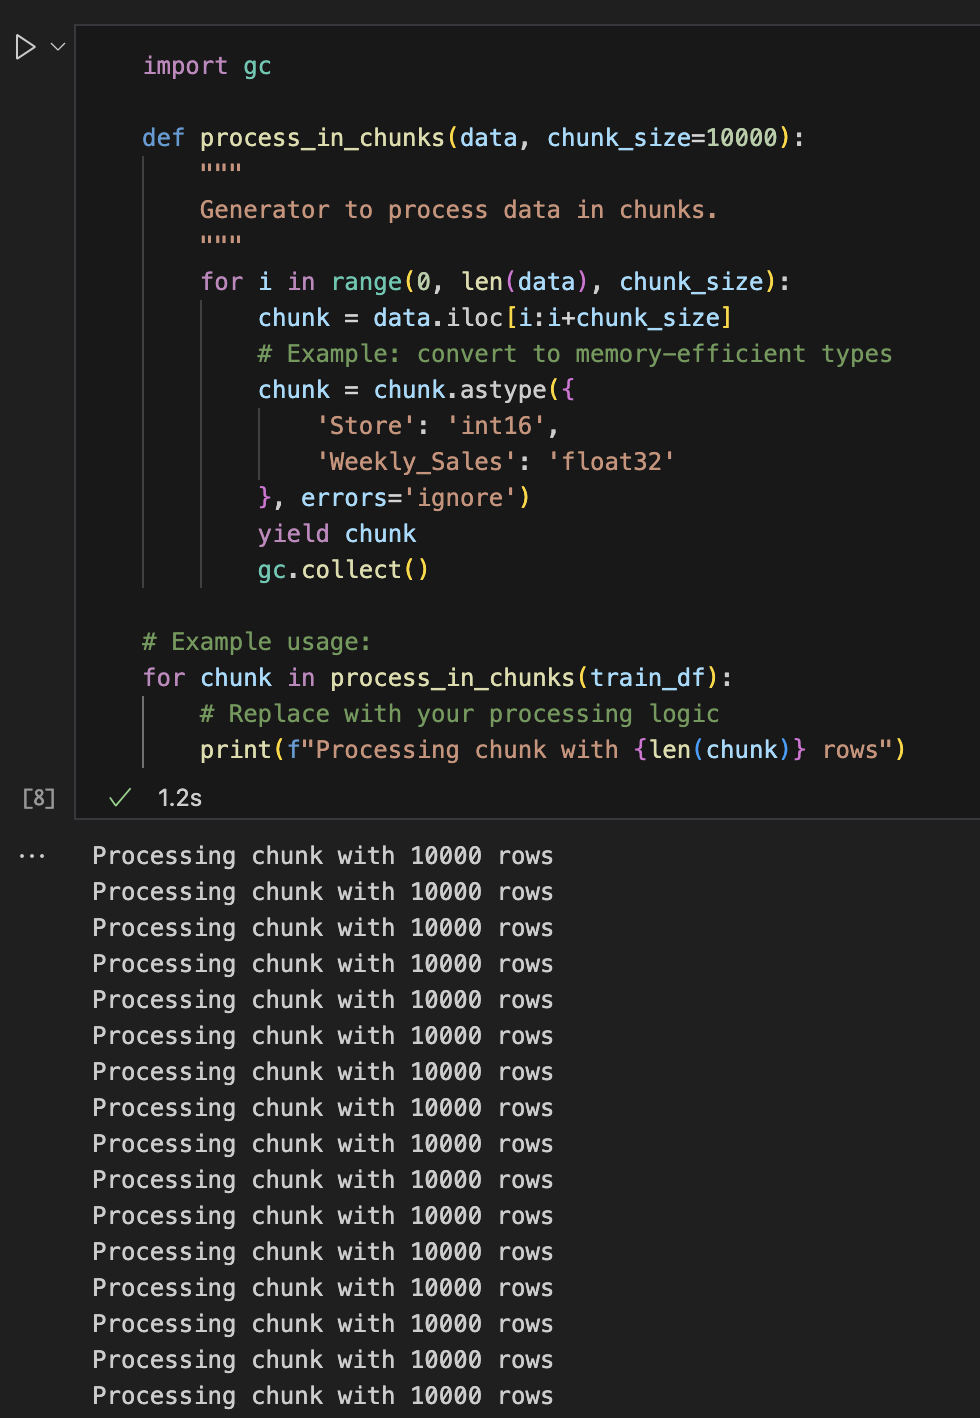
\includegraphics[width=0.9\textwidth]{Images/08Troubleshooting/MemoryManagement.png}
	\caption{Memory Management and Optimization Interface}
	\label{fig:memory_management}
\end{figure}

\section{Prediction Issues}

\subsection{Prediction Generation Failures}

\subsubsection{Forecast Generation Errors}

\textbf{Problem}: Prediction generation fails with loaded model

\textbf{Symptoms}:
\begin{itemize}
	\item "Error generating predictions" messages
	\item NaN values in forecast results
	\item Unrealistic forecast values
\end{itemize}

\textbf{Diagnostic Steps}:
\begin{lstlisting}[language=python,basicstyle=\color{blue}]
	# Test model prediction manually
	try:
	if model_type == "Auto ARIMA":
	predictions = model.predict(n_periods=4)
	else:
	predictions = model.forecast(4)
	print("Predictions:", predictions)
	except Exception as e:
	print(f"Prediction error: {e}")
\end{lstlisting}

\textbf{Solution}:
\begin{enumerate}
	\item Verify model was trained successfully
	\item Check model type matches prediction method
	\item Ensure model has sufficient training data
	\item Retrain model if necessary
	\item Check for data preprocessing consistency
\end{enumerate}

\subsection{Result Interpretation Issues}

\subsubsection{Unexpected Forecast Values}

\textbf{Problem}: Forecasts seem unrealistic or inconsistent

\textbf{Symptoms}:
\begin{itemize}
	\item All negative predictions
	\item Extremely large prediction values
	\item No seasonal patterns visible
\end{itemize}

\textbf{Analysis Steps}:
\begin{itemize}
	\item Remember predictions are week-over-week changes, not absolute sales
	\item Check training data for similar patterns
	\item Compare with historical sales changes
	\item Verify model performance metrics (WMAE)
\end{itemize}

\textbf{Solution}:
\begin{enumerate}
	\item Review model training performance
	\item Consider retraining with different parameters
	\item Validate training data quality
	\item Compare multiple model types
	\item Consult domain expertise for reasonableness
\end{enumerate}

\section{Test Suite Validation}

\subsection{Using Pytest for Troubleshooting}

\subsubsection{Running Diagnostic Tests}

\textbf{Comprehensive Test Execution}:
\begin{lstlisting}[language=bash,basicstyle=\color{blue}]
	# Run all tests with verbose output
	pytest testWalmartSalesTraining.py -v
	pytest testWalmartSalesPrediction.py -v
	
	# Run specific test categories
	pytest -k "test_load" -v  # Only model loading tests
	pytest -k "test_predict" -v  # Only prediction tests
	
	# Run tests with detailed output
	pytest --tb=long -v  # Long traceback format
	pytest --tb=short -v  # Short traceback format
	
	# Run tests and stop on first failure
	pytest -x -v
	
	# Generate test coverage report
	pytest --cov=walmartSalesTrainingCore --cov=walmartSalesPredictionCore
\end{lstlisting}

\textbf{Interpreting Test Results}:
\begin{itemize}
	\item \textbf{All tests PASSED}: System is functioning correctly
	\item \textbf{Specific test FAILED}: Identifies exact problem area
	\item \textbf{Import errors}: Package installation issues
	\item \textbf{Timeout errors}: Performance or resource issues
\end{itemize}

\begin{figure}[H]
	\centering
%	\includegraphics[width=0.9\textwidth]{Images/08_Troubleshooting/PytestValidation.png}
	\caption{Pytest Validation and Diagnostic Results}
	\label{fig:pytest_validation}
\end{figure}

\subsubsection{Custom Diagnostic Tests}

\textbf{Create Custom Test Scripts}:
\begin{figure}[H]
	\centering
		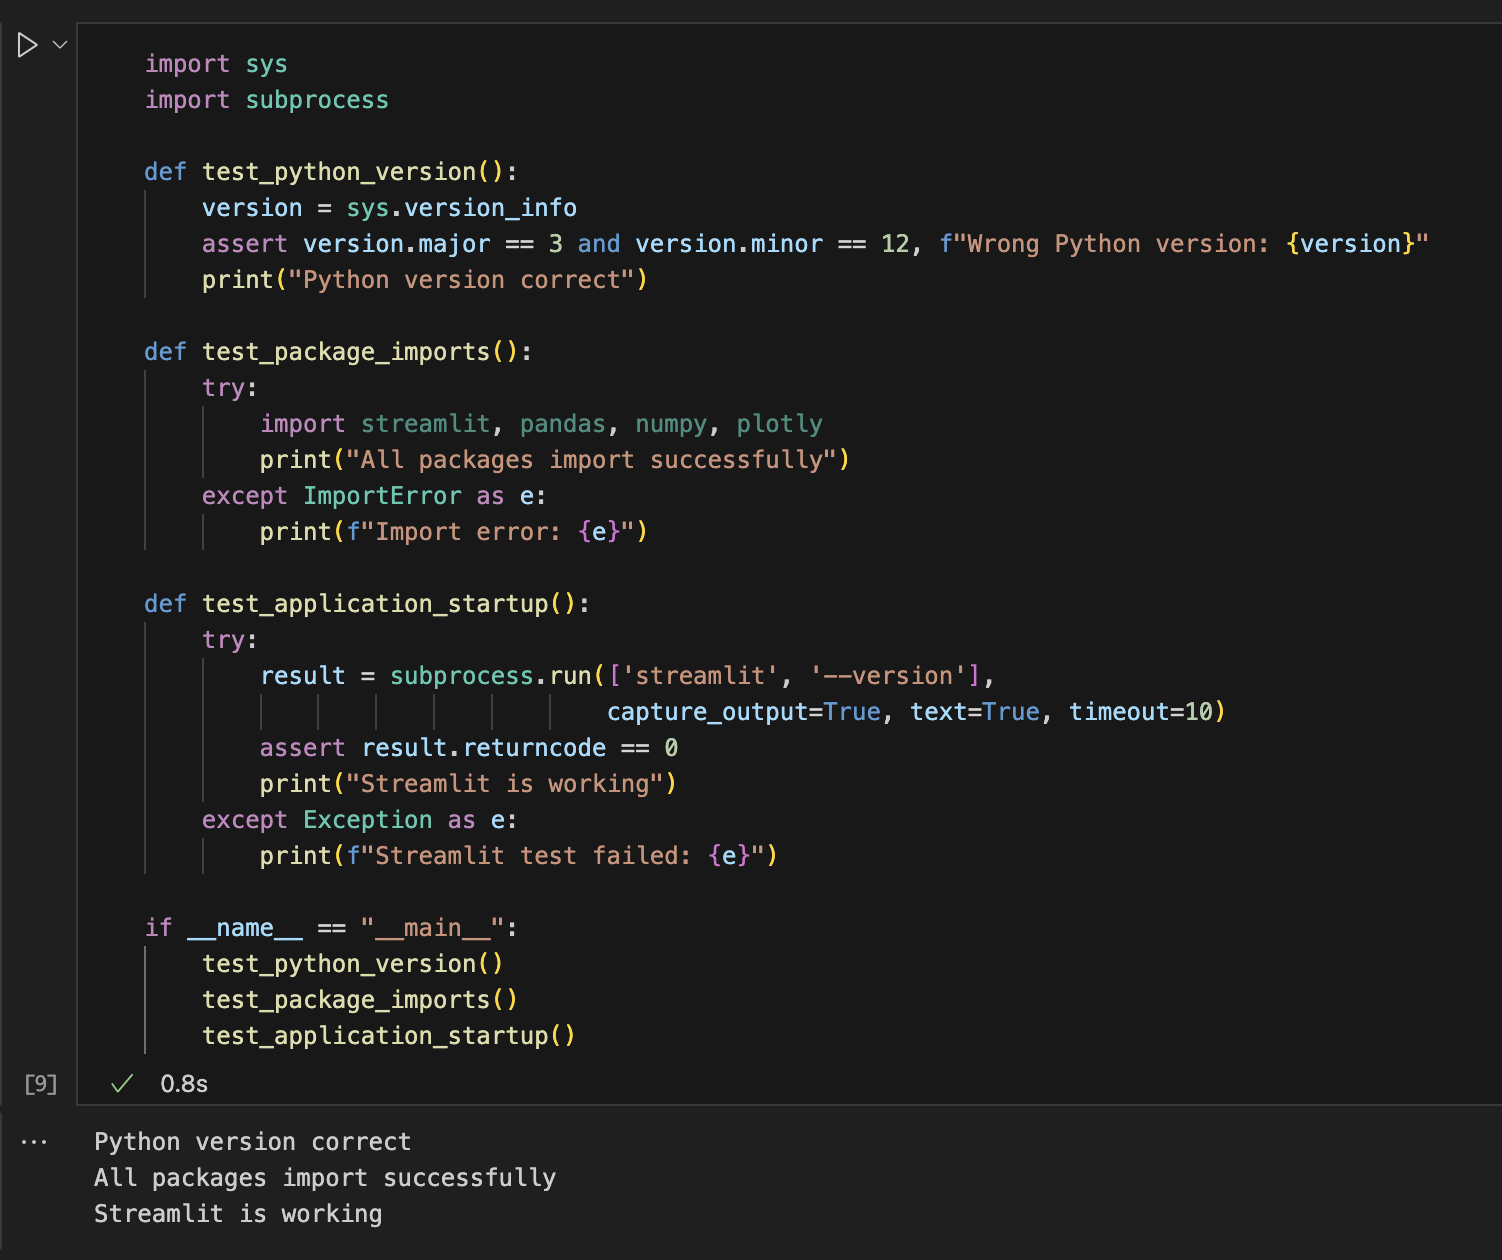
\includegraphics[width=1\textwidth]{Images/08Troubleshooting/CustomTestScripts.png}
	\caption{Pytest Validation and Diagnostic Results}
	\label{fig:CustomTestScripts}
\end{figure}

\section{Advanced Troubleshooting}

\subsection{Log Analysis}

\subsubsection{Enabling Debug Logging}

\textbf{Enhanced Logging Configuration}:
\begin{figure}[H]
	\centering
		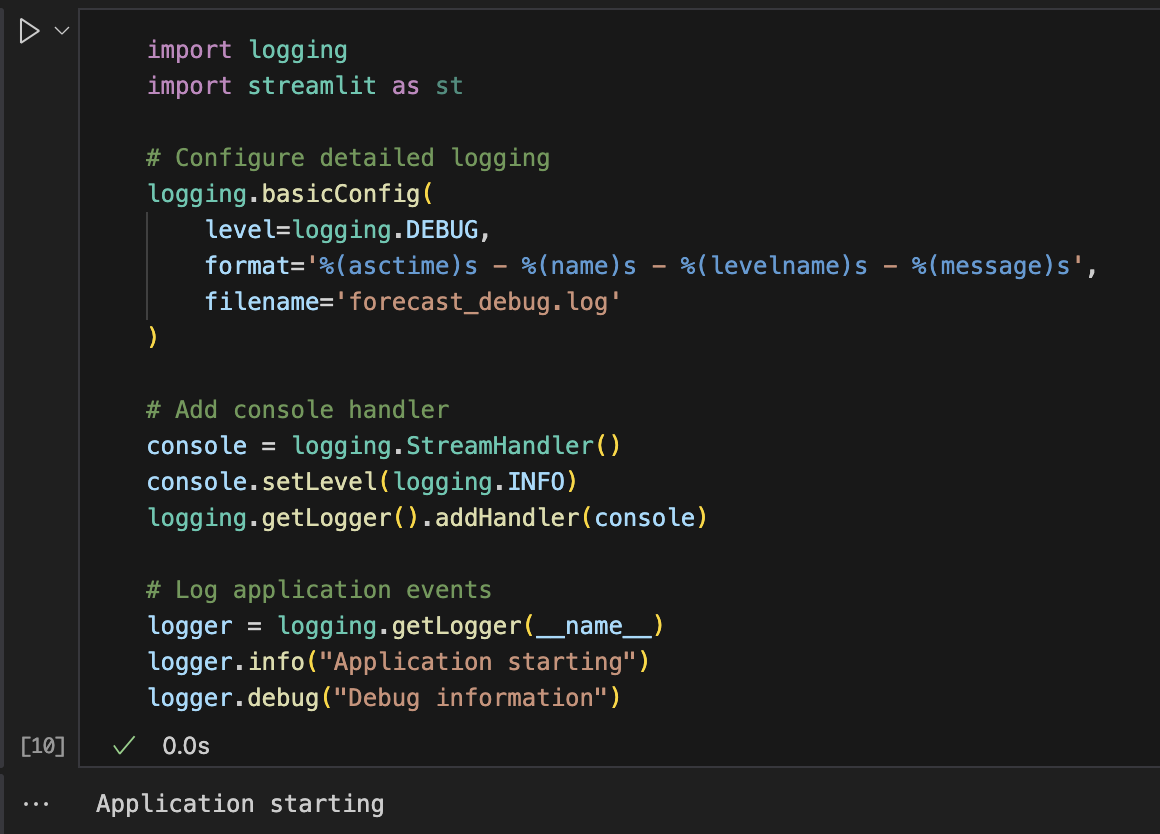
\includegraphics[width=1\textwidth]{Images/08Troubleshooting/Logging.png}
	\caption{Pytest Validation and Diagnostic Results}
	\label{fig:Logging}
\end{figure}

\subsection{Performance Profiling}

\section{Emergency Recovery Procedures}

\subsection{System Recovery}

\subsubsection{Complete Environment Reset}

\textbf{Nuclear Option - Full Reset}:
\begin{figure}[H]
	\centering
		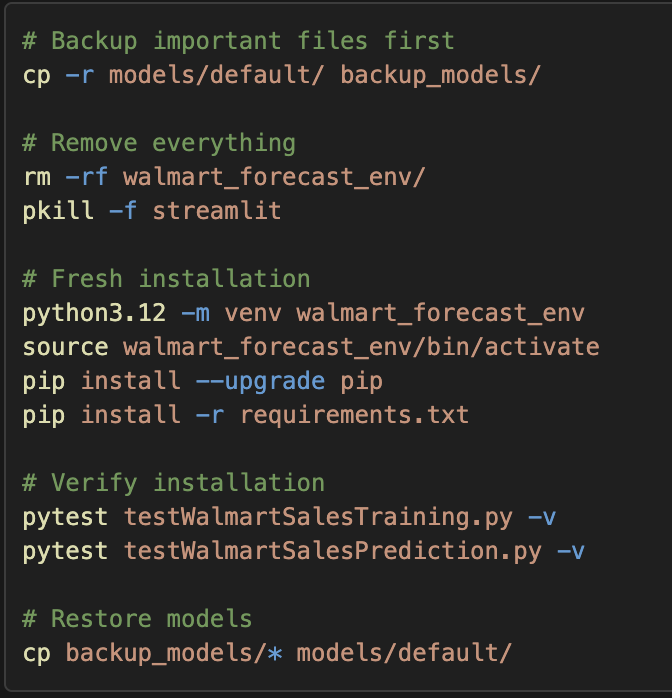
\includegraphics[width=0.9\textwidth]{Images/08Troubleshooting/FullReset.png}
	\caption{Pytest Validation and Diagnostic code}
	\label{fig:FullReset}
\end{figure}
\subsection{Data Recovery}

\subsubsection{Recovering Lost Work}

\textbf{Model Recovery Steps}:
\begin{enumerate}
	\item Check models/default/ directory for saved models
	\item Look in backup directories created by maintenance procedures
	\item Re-download models from cloud applications if available
	\item Retrain models using original training data
	\item Document lessons learned to prevent recurrence
\end{enumerate}

\section{Getting Additional Help}

\subsection{Documentation Resources}

\textbf{Internal Documentation}:
\begin{itemize}
	\item This user manual for comprehensive guidance
	\item Code comments in application files
	\item Test files for expected behavior examples
	\item README files for quick reference
\end{itemize}

\textbf{External Resources}:
\begin{itemize}
	\item Streamlit documentation: \url{https://docs.streamlit.io/}
	\item pandas documentation: \url{https://pandas.pydata.org/docs/}
	\item pmdarima documentation: \url{https://alkaline-ml.com/pmdarima/}
	\item statsmodels documentation: \url{https://www.statsmodels.org/}
\end{itemize}

\subsection{Community Support}

\textbf{Online Communities}:
\begin{itemize}
	\item Stack Overflow for programming questions
	\item Streamlit Community Forum
	\item Reddit r/MachineLearning and r/Python
	\item GitHub Issues for package-specific problems
\end{itemize}

\section{Troubleshooting Quick Reference}

\begin{table}[H]
	\centering
	\begin{tabularx}{\textwidth}{|X|X|X|}
		\hline
		\textbf{Problem} & \textbf{Quick Check} & \textbf{Quick Fix} \\
		\hline
		App won't start & Python version & python3.12 -m venv env \\
		Import errors & Virtual env active & pip install -r requirements.txt \\
		Port in use & Check processes & pkill -f streamlit \\
		Upload fails & File size/format & Check file < 200MB, .csv/.pkl \\
		Model won't load & File integrity & Retrain and re-export model \\
		Slow training & Resource usage & Reduce parameter ranges \\
		Cloud timeout & Session length & Download results frequently \\
		Tests fail & Environment & Run pytest -v for details \\
		\hline
	\end{tabularx}
	\caption{Troubleshooting Quick Reference Guide}
	\label{tab:troubleshooting_reference}
\end{table}


This comprehensive troubleshooting guide addresses the most common issues users encounter with the Walmart Sales Forecasting System. The next chapter provides additional help resources and support information.